%
%
\pgfplotsset{colormap={cubicyf}{
rgb = (0.5151, 0.0482, 0.66969999999999996)
rgb = (0.52071100000000003, 0.16895499999999999, 0.80057400000000001)
rgb = (0.49369400000000002, 0.27859600000000001, 0.91182399999999997)
rgb = (0.44002599999999997, 0.369475, 0.98497800000000002)
rgb = (0.39893200000000001, 0.45759300000000003, 0.98705299999999996)
rgb = (0.35065099999999999, 0.54064400000000001, 0.92960799999999999)
rgb = (0.29882700000000001, 0.61562499999999998, 0.85772899999999996)
rgb = (0.239928, 0.68506100000000003, 0.76953099999999997)
rgb = (0.22883200000000001, 0.73934900000000003, 0.67328699999999997)
rgb = (0.263297, 0.78608, 0.56998800000000005)
rgb = (0.29810700000000001, 0.82833699999999999, 0.46021400000000001)
rgb = (0.33091999999999999, 0.86407100000000003, 0.35267399999999999)
rgb = (0.38306000000000001, 0.898169, 0.28730899999999998)
rgb = (0.49023, 0.91748099999999999, 0.30796099999999998)
rgb = (0.62372000000000005, 0.92602600000000002, 0.33230900000000002)
rgb = (0.71745800000000004, 0.92527000000000004, 0.342476)
rgb = (0.80000000000000004, 0.92549999999999999, 0.35289999999999999)
}}
\pgfplotsset{colormap={rdoryl}{
rgb(0)=(1, 1, 0.80000000000000004)
rgb(1)=(1, 0.96678200000000003, 0.71879999999999999)
rgb(2)=(1, 0.93134899999999998, 0.63218799999999997)
rgb(3)=(0.998139, 0.89219499999999996, 0.54929600000000001)
rgb(4)=(0.99617100000000003, 0.85282599999999997, 0.46662100000000001)
rgb(5)=(0.99607800000000002, 0.77780899999999997, 0.38394499999999998)
rgb(6)=(0.99607800000000002, 0.70103800000000005, 0.30126900000000001)
rgb(7)=(0.99418700000000004, 0.62805100000000003, 0.26777400000000001)
rgb(8)=(0.99221800000000004, 0.55521699999999996, 0.23627799999999999)
rgb(9)=(0.99024999999999996, 0.43280299999999999, 0.20096900000000001)
rgb(10)=(0.98828099999999997, 0.30878899999999998, 0.16553599999999999)
rgb(11)=(0.94017700000000004, 0.20592099999999999, 0.137793)
rgb(12)=(0.89096500000000001, 0.10356, 0.110235)
rgb(13)=(0.81656300000000004, 0.051580000000000001, 0.12918099999999999)
rgb(14)=(0.741761, 0.00040000000000000002, 0.148866)
rgb(15)=(0.62203799999999998, 0, 0.14902000000000001)
rgb(16)=(0.50196099999999999, 0, 0.14902000000000001)
}}
%
\begin{tikzpicture}[
    font=\small,
    image/.style={inner sep=0, outer sep=0, node distance = 0.25cm and 0.25cm},
    label/.style={fill=white, anchor=south west, xshift=1mm, yshift=1mm}
]

    % place image in node
    \node[image] (image1)
    {
        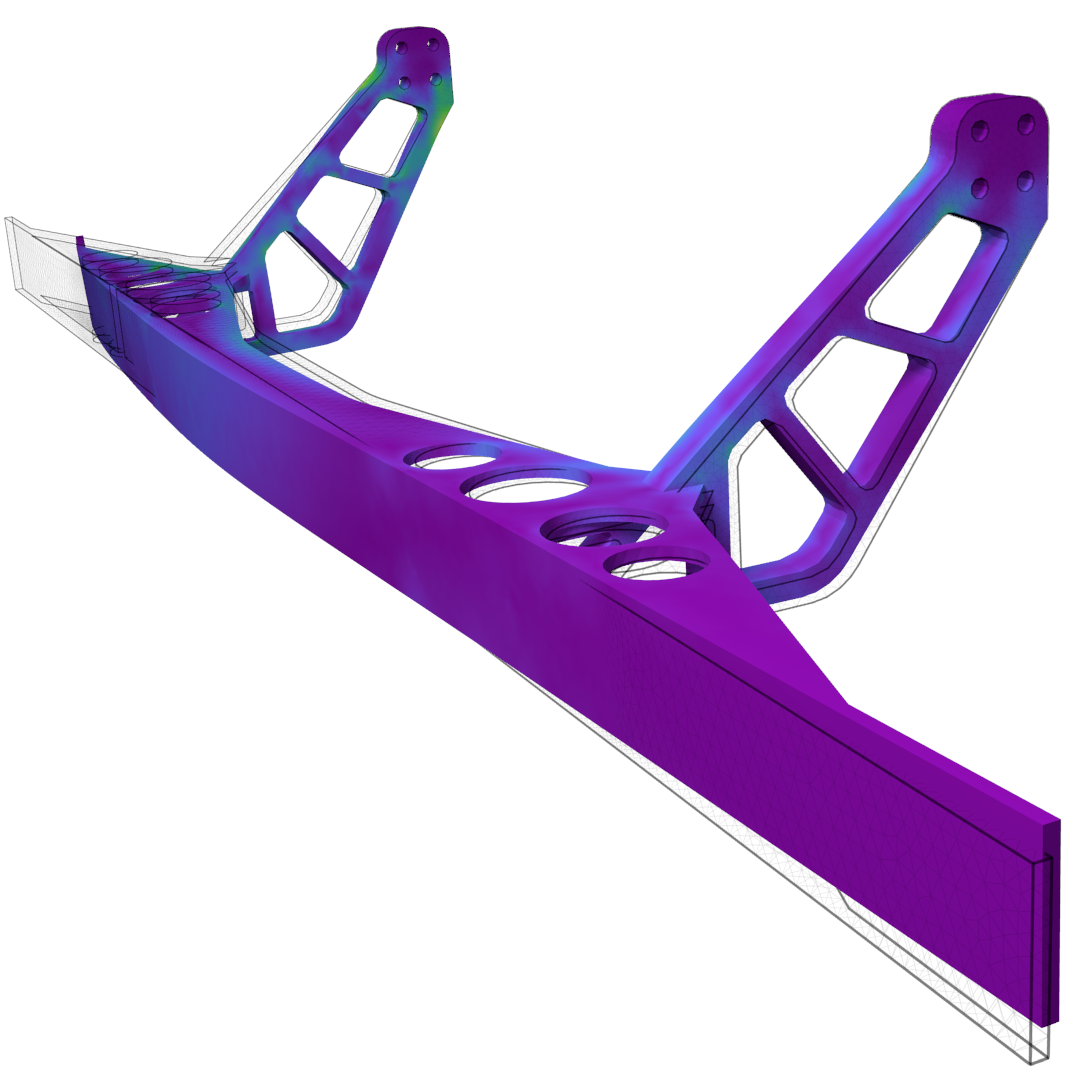
\includegraphics[width=0.5\figurewidth - 0.125cm - 1cm]{figures/truck_bumper_deformation}%
    };

    % place next image to the right with a little space in between
    \node[image, right=of image1] (image2)
    {
        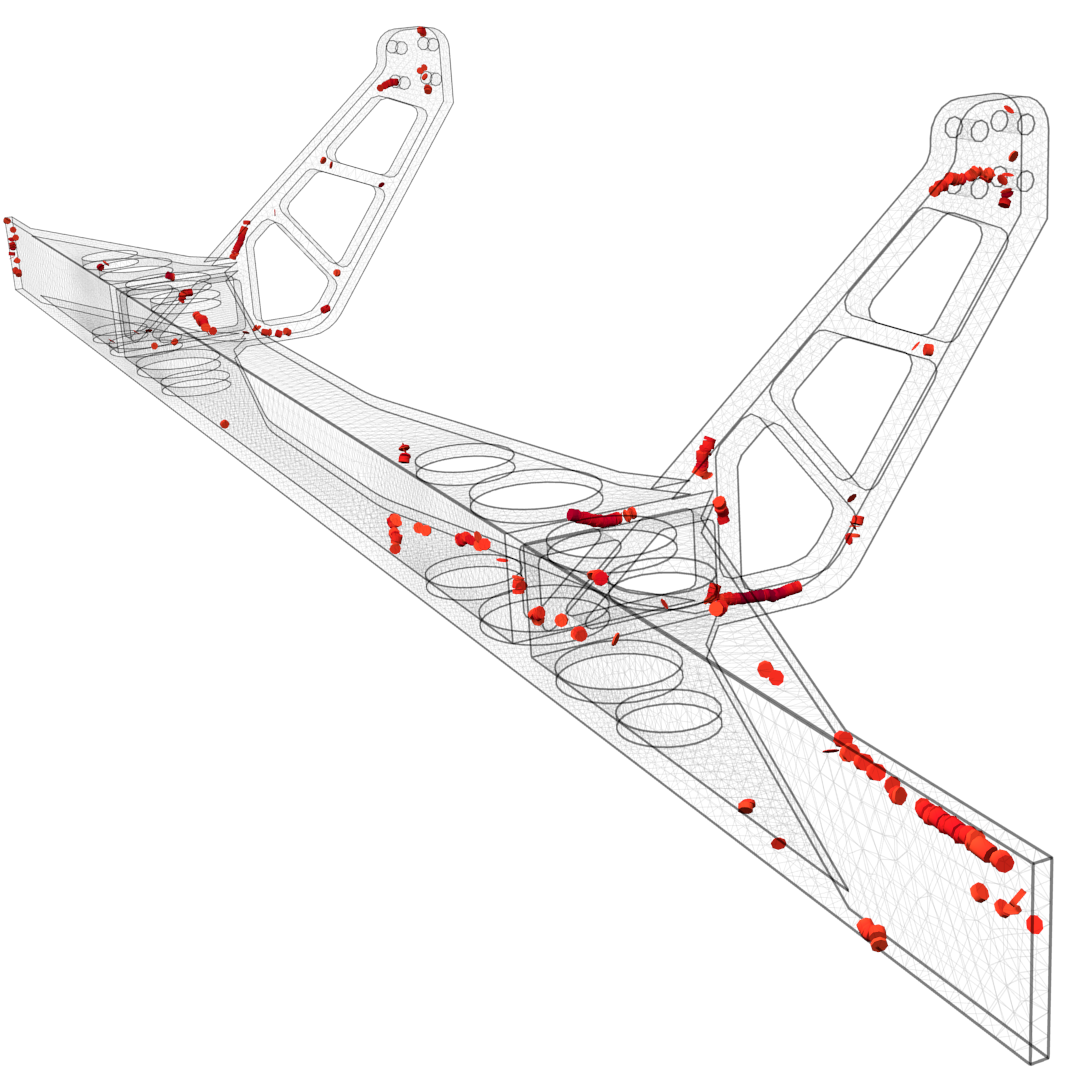
\includegraphics[width=0.5\figurewidth - 0.125cm - 1cm]{figures/truck_bumper_lines}%
    };
    % create new coordinate system on image2:
    \begin{scope}[
        shift=(image2.south west), % origin is lower left corner
        x={($(image2.south east)-(image2.south west)$)}, % x axis is lower side
        y={($(image2.north west)-(image2.south west)$)}] % y axis is left side
        % uncomment the following three lines to show a helper grid that helps
        % with finding coordinates
        % \draw[help lines,xstep=.1,ystep=.1] (0,0) grid (1,1);
        % \foreach \x in {0,1,...,9} { \node [anchor=north] at (\x/10,0) {\scriptsize 0.\x}; }
        % \foreach \y in {0,1,...,9} { \node [anchor=east] at (0,\y/10) {\scriptsize 0.\y}; }
        % draw stuff on image
        % (0, 0) is lower left corner, (1, 1) is upper right
        \draw [thin, -] (0.55, 0.535) -- (0.55, 0.6) node [anchor=south] {\normalsize \textbf{$1$}};
        \draw [thin, -] (0.72, 0.435) -- (0.8, 0.4) node [anchor=west] {\normalsize \textbf{$2$}};
    \end{scope}

    \node[image, below=of image1] (image3)
    {
        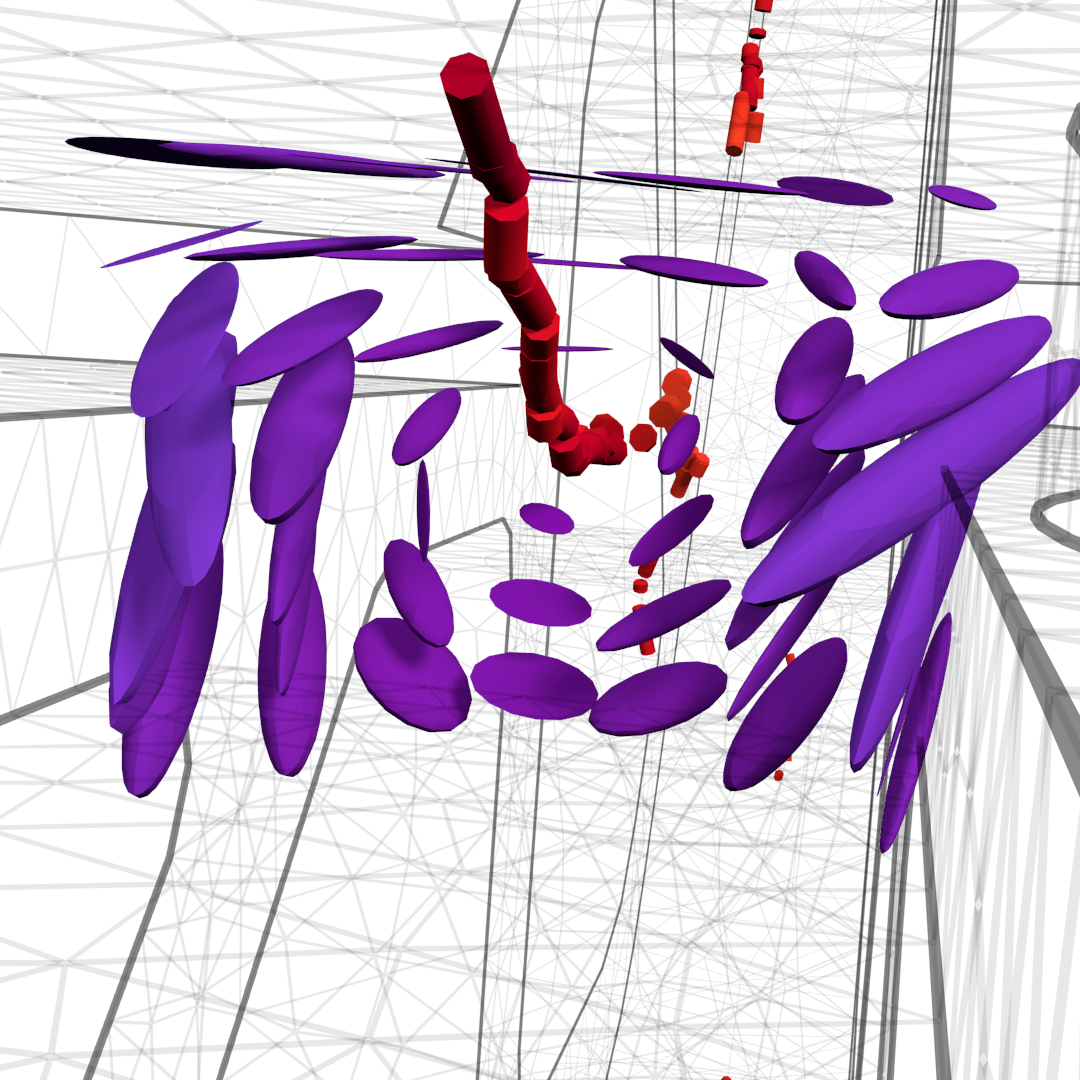
\includegraphics[width=0.5\figurewidth - 0.125cm - 1cm]{figures/truck_bumper_detail2}%
    };
    % place a text on the lower left corner of image3
    \node [label] at (image3.south west) {\large \textbf{$1$}};

    \node[image, right=of image3] (image4)
    {
        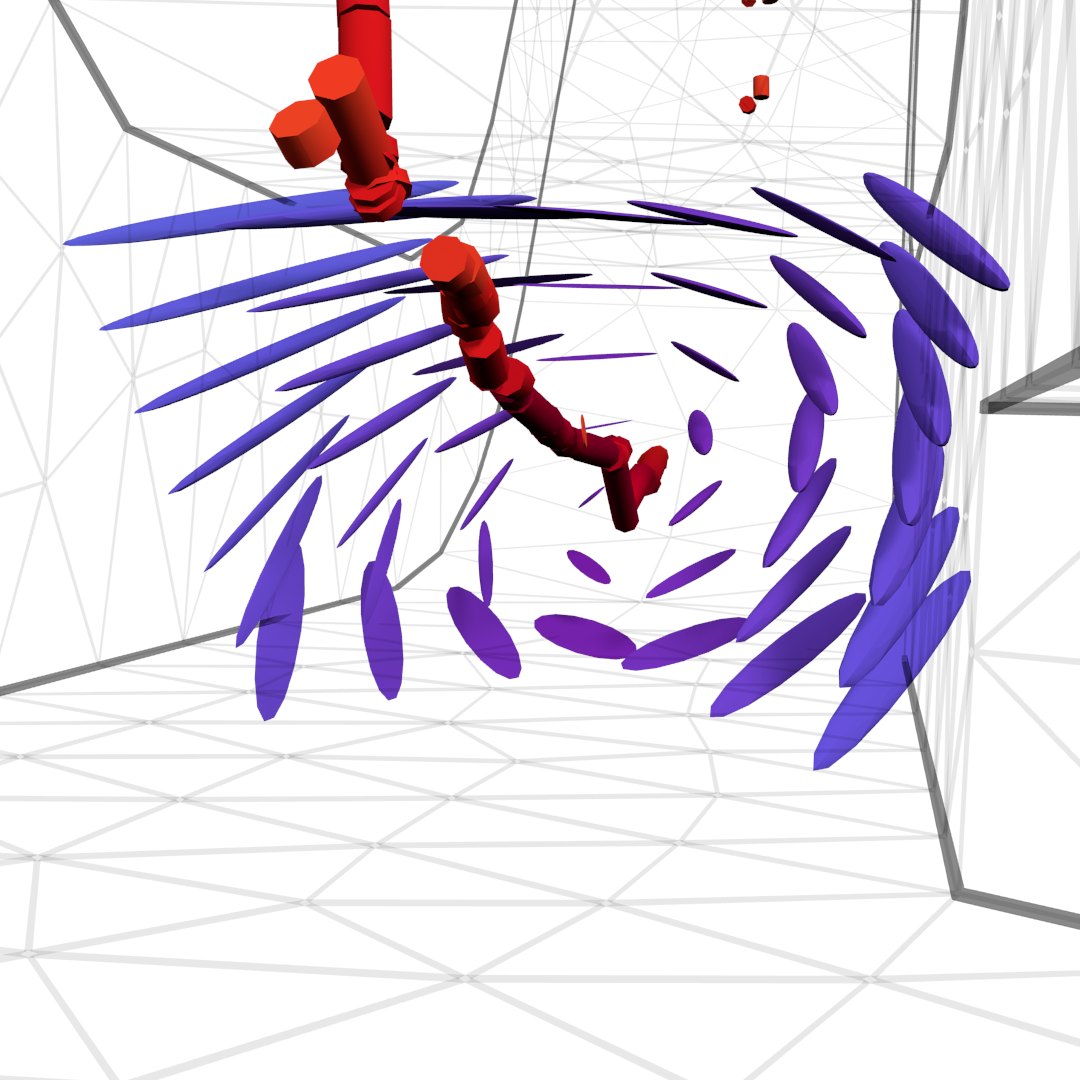
\includegraphics[width=0.5\figurewidth - 0.125cm - 1cm]{figures/truck_bumper_detail1}%
    };
    \node [label] at (image4.south west) {\large \textbf{$2$}};


    \clip (image1.north west) -- ($(image2.north east) + (2.25cm, 0)$) --
    ($(image4.south east) + (2.25cm, -2mm)$) -- (image3.south west) -- cycle;

    \node[anchor=south west, xshift=-0.6cm, yshift=-3.5mm] (stabscale) at (image4.south east){
        \begin{axis}[
            scale only axis,
            height=2.8cm,
            hide axis,
            domain=1:20,
            colorbar,
            colorbar/width=0.25cm,
            colormap name={rdoryl},
            point meta min=1.5, point meta max=15,
            colorbar style={
                title=$\log(s)$,
                scaled ticks=false,
                ytick={1.5, 15}
            }]
        \end{axis}
    };
    \node[anchor=south west, xshift=1.3mm] at (stabscale.north west){
        \begin{axis}[
            scale only axis,
            height=2.8cm,
            hide axis,
            domain=1:20,
            colorbar,
            colorbar/width=0.25cm,
            colormap name={cubicyf},
            point meta min=0, point meta max=9e6,
            colorbar style={
                title=$\sigma_{\textnormal{vM}}$,
                scaled ticks=false,
                ytick={0, 9e6}
            }]
        \end{axis}
    };

\end{tikzpicture}